% main.tex — Rapport de Génie Logiciel — SaaS Directory

% HEEC Marrakech — 2026

\documentclass[12pt,a4paper]{article}



% ======================== PACKAGES ========================

\usepackage{fontspec}

\setmainfont{Times New Roman}

\usepackage{polyglossia}

\setmainlanguage{french}



\usepackage{geometry}

\geometry{a4paper, top=2.5cm, bottom=2.5cm, left=2.5cm, right=2cm}



\usepackage{graphicx}

\usepackage{xcolor}

\usepackage{booktabs}

\usepackage{longtable}

\usepackage{array}

\usepackage{multirow}

\usepackage{enumitem}

\usepackage{fancyhdr}

\usepackage{titlesec}

\usepackage{setspace}

\usepackage{float}

\usepackage{caption}

\usepackage{subcaption}

\usepackage{listings}

\usepackage{tcolorbox}

\tcbuselibrary{skins,breakable}



% Math (must load before hyperref)
\usepackage{amsmath}

% hyperref MUST be loaded last

\usepackage[
    colorlinks=true,
    linkcolor=HEECnavy,
    citecolor=darkgray,
    urlcolor=blue,
    bookmarks=true,
    bookmarksnumbered=true,
    unicode=true,
    pdftitle={Rapport de Genie Logiciel --- SaaS Directory},
    pdfauthor={Omar SARSAR, Iliass HARIZ}
]{hyperref}



% ======================== COLORS ========================

\definecolor{HEECnavy}{RGB}{27,58,107}

\definecolor{HEECgold}{RGB}{212,175,55}

\definecolor{HEECburgundy}{RGB}{107,39,55}

\definecolor{HEECdark}{RGB}{26,32,44}

\definecolor{HEEClight}{RGB}{113,128,150}

\definecolor{HEECmid}{RGB}{74,85,104}

\definecolor{BoxBg}{RGB}{240,245,250}

\definecolor{CodeBg}{RGB}{245,245,245}



% ======================== SPACING ========================

\onehalfspacing

\setlength{\parindent}{0pt}

\setlength{\parskip}{0.5em}



% ======================== HEADERS/FOOTERS ========================

\pagestyle{fancy}

\fancyhf{}

\fancyhead[R]{\small\textit{SaaS Directory — Rapport de Génie Logiciel}}

\fancyfoot[C]{\thepage}

\renewcommand{\headrulewidth}{0.4pt}

\renewcommand{\footrulewidth}{0pt}



% ======================== SECTION STYLING ========================

\titleformat{\section}
  {\normalfont\Large\bfseries\color{white}}
  {}
  {0pt}
  {}
  [\vspace{-1em}]

\titlespacing*{\section}{0pt}{24pt}{12pt}

\newcommand{\sectioncolor}{%

  \titleformat{\section}{\normalfont\Large\bfseries\color{white}}{}{0pt}{}[\vspace{-1em}]%

}



\titleformat{\subsection}
  {\normalfont\large\bfseries\color{HEECnavy}}
  {\thesubsection}{1em}{}

\titlespacing*{\subsection}{0pt}{18pt}{6pt}



\titleformat{\subsubsection}
  {\normalfont\normalsize\bfseries\color{HEECburgundy}}
  {\thesubsubsection}{1em}{}

\titlespacing*{\subsubsection}{0pt}{12pt}{6pt}



% ======================== TCOLORBOX DEFINITIONS ========================

\newtcolorbox{definitionbox}[1][]{
  colback=BoxBg,
  colframe=HEECnavy,
  boxrule=0pt,
  leftrule=4pt,
  arc=0pt,
  left=8pt,
  right=8pt,
  top=6pt,
  bottom=6pt,
  breakable,
  fonttitle=\bfseries\color{HEECnavy},
  #1
}



\newtcolorbox{codebox}{
  colback=CodeBg,
  colframe=HEECmid,
  boxrule=0pt,
  leftrule=2pt,
  arc=0pt,
  left=8pt,
  right=8pt,
  top=4pt,
  bottom=4pt,
  breakable
}



% ======================== LISTINGS CONFIG ========================

\lstset{
  basicstyle=\ttfamily\small,
  backgroundcolor=\color{CodeBg},
  frame=none,
  breaklines=true,
  breakatwhitespace=true,
  showstringspaces=false,
  tabsize=2,
  xleftmargin=1em,
  xrightmargin=1em
}



% ======================== DOCUMENT START ========================

\begin{document}



% ======================== COVER PAGE ========================

\thispagestyle{empty}

\begin{center}

\vspace*{1cm}



{\color{HEECgold}\rule{0.8\textwidth}{1.5pt}}



\vspace{0.8cm}



{\Huge\bfseries\color{HEECnavy} HEEC}



\vspace{0.3cm}



{\Large\color{HEECdark} École des Hautes Études Économiques Commerciales\\

et d'Ingénierie de Marrakech}



\vspace{0.8cm}



{\color{HEECgold}\rule{0.8\textwidth}{1.5pt}}



\vspace{1.5cm}



{\LARGE\bfseries\color{HEECnavy} RAPPORT DE GÉNIE LOGICIEL\\

ET CONDUITE DE PROJET}



\vspace{0.8cm}



{\large\color{HEECburgundy} Application des concepts de Génie Logiciel\\

et de Conduite de Projet au développement de\\[0.5em]

\textbf{SaaS Directory}}



\vspace{1.5cm}



{\color{HEECgold}\rule{0.6\textwidth}{1pt}}



\vspace{1cm}



{\large\bfseries Présenté par :}



\vspace{0.3cm}



{\large\bfseries\color{HEECnavy} Omar SARSAR\\

Iliass HARIZ}



\vspace{2cm}



{\Huge\bfseries\color{HEECgold} 2026}



\vspace{0.5cm}



{\color{HEECgold}\rule{0.8\textwidth}{1.5pt}}



\end{center}



\newpage



% ======================== DÉDICACE ========================

\thispagestyle{empty}

\vspace*{8cm}

\begin{center}

{\large\textit{Nous dédions ce travail à nos familles pour leur soutien indéfectible,\\
à nos enseignants pour leur guidance et leurs enseignements,\\
et à tous ceux qui croient en l'innovation technologique au service de la communauté.}}

\end{center}

\newpage



% ======================== REMERCIEMENTS ========================

\thispagestyle{empty}

\section*{Remerciements}

\addcontentsline{toc}{section}{Remerciements}



Nous tenons à exprimer notre profonde gratitude envers l'ensemble de nos enseignants qui nous ont accompagnés tout au long de notre parcours académique. Leurs conseils avisés, leur patience et leur exigence ont été des facteurs déterminants dans la réussite de ce projet.



Nous remercions également nos camarades de promotion pour les échanges enrichissants et l'entraide collective qui ont contribué à notre progression.



\newpage



% ======================== RÉSUMÉ ========================

\thispagestyle{empty}

\section*{Résumé}

\addcontentsline{toc}{section}{Résumé}



Ce rapport présente l'application systématique des concepts de Génie Logiciel et de Conduite de Projet au développement de \textbf{SaaS Directory}, une plateforme de marketplace dédiée aux produits logiciels en mode SaaS. Le projet a été réalisé avec une stack technologique moderne comprenant Next.js 16.2.4, React 19.2.4, TypeScript, Tailwind CSS v4, Drizzle ORM 0.45.2, PostgreSQL et Better Auth 1.6.9.



L'étude couvre l'ensemble des neuf chapitres du cours de Génie Logiciel : rappels fondamentaux, généralités, cycle de vie du logiciel, démarche de conception, normalisation, tests, gestion de projet, analyse des risques et conduite du changement. Chaque concept théorique est illustré par sa mise en Å“uvre concrète dans le projet.



Le rapport inclut une estimation du coût par la méthode COCOMO appliquée à la base de code réelle de 12 166 lignes, une analyse des risques liés aux breaking changes de Next.js 16.2.4, ainsi qu'une présentation détaillée de la gestion des versions via Git et des migrations Drizzle ORM.



\vspace{0.5cm}

\noindent\textbf{Mots-clés :} Génie Logiciel, Conduite de Projet, Next.js, React, Drizzle ORM, PostgreSQL, COCOMO, Cycle de Vie, UML, Normalisation, Tests Logiciels, Gestion des Risques.



\newpage



% ======================== ABSTRACT ========================

\thispagestyle{empty}

\section*{Abstract}

\addcontentsline{toc}{section}{Abstract}



This report presents the systematic application of Software Engineering and Project Management concepts to the development of \textbf{SaaS Directory}, a marketplace platform dedicated to SaaS software products. The project was built using a modern technology stack including Next.js 16.2.4, React 19.2.4, TypeScript, Tailwind CSS v4, Drizzle ORM 0.45.2, PostgreSQL, and Better Auth 1.6.9.



The study covers all nine chapters of the Software Engineering course: fundamental recalls, general concepts, software life cycle, design methodology, standardization, testing, project management, risk analysis, and change management. Each theoretical concept is illustrated by its concrete implementation in the project.



The report includes a COCOMO cost estimation applied to the actual codebase of 12,166 lines, a risk analysis related to Next.js 16.2.4 breaking changes, and a detailed presentation of version control via Git and Drizzle ORM migrations.



\vspace{0.5cm}

\noindent\textbf{Keywords:} Software Engineering, Project Management, Next.js, React, Drizzle ORM, PostgreSQL, COCOMO, Life Cycle, UML, Standardization, Software Testing, Risk Management.



\newpage



% ======================== TABLE OF CONTENTS ========================

\tableofcontents

\newpage



% ======================== LIST OF FIGURES ========================

\listoffigures

\newpage



% ======================== LIST OF TABLES ========================

\listoftables

\newpage



% ======================== INTRODUCTION ========================

\section*{Introduction Générale}

\addcontentsline{toc}{section}{Introduction Générale}



Dans un monde de plus en plus numérisé, le développement de logiciels est devenu une discipline complexe qui exige rigueur, méthodologie et gestion efficace des ressources. Le Génie Logiciel (GL) et la Conduite de Projet fournissent le cadre théorique et pratique nécessaire pour mener à bien des projets logiciels de qualité, dans les délais et budgets impartis.



Ce rapport a pour objectif de démontrer l'application concrète des concepts théoriques du Génie Logiciel et de la Conduite de Projet au développement de \textbf{SaaS Directory}, une application web moderne permettant aux créateurs de logiciels de lancer, promouvoir et vendre leurs produits SaaS.



SaaS Directory est une application web moderne permettant aux créateurs de logiciels de lancer, promouvoir et vendre leurs produits SaaS (Software as a Service). L'application offre un marketplace où les utilisateurs peuvent découvrir des outils logiciels, voter pour leurs produits préférés, interagir via des commentaires et une messagerie temps réel, et souscrire à des plans d'abonnement Free ou Pro.



Le projet a été réalisé avec une stack technologique contemporaine et cohérente : Next.js 16.2.4 (framework React avec App Router), React 19.2.4, TypeScript 5, Tailwind CSS v4, Drizzle ORM 0.45.2 (ORM type-safe pour PostgreSQL), Better Auth 1.6.9 (authentification complète avec OAuth et 2FA), Redis (cache et Pub/Sub pour la messagerie temps réel), et Playwright 1.59.1 pour les tests end-to-end.



\textbf{Le codebase} compte exactement \textbf{20 tables} dans le schéma Drizzle ORM, \textbf{12 166 lignes de code} réparties sur \textbf{108 fichiers} TypeScript/TSX, avec \textbf{4 migrations} versionnées (0000 à 0003). Le projet est versionné sur Git avec une branche \texttt{master} principale et des branches de fonctionnalités.



Ce rapport s'articule autour de neuf chapitres principaux. Le premier chapitre présente les rappels fondamentaux sur les concepts de base. Le deuxième traite des généralités du Génie Logiciel et de ses principes. Le troisième décrit les modèles de cycle de vie. Le quatrième expose la démarche de conception avec UML. Le cinquième aborde la normalisation. Le sixième détaille les stratégies de tests. Le septième présente la gestion de projet et l'estimation COCOMO. Le huitième analyse les risques. Le neuvième et dernier chapitre traite de la conduite du changement.



\newpage



% ======================== CHAPTERS ========================

% Chapitre 1 : Rappels


\section{Chapitre 1 : Rappels}





\subsection{Définitions Fondamentales}





Avant d'aborder les concepts avancés du Génie Logiciel, il est essentiel de poser les bases terminologiques et conceptuelles sur lesquelles repose l'ensemble de la discipline.





\subsubsection{Logiciel et Application}





Un \textbf{logiciel} est défini comme un ensemble de programmes, procédures, règles et documentations relatifs au fonctionnement d'un ensemble de traitements d'informations. Cette définition englobe non seulement le code source, mais aussi la documentation technique, les manuels utilisateurs, et les spécifications fonctionnelles.





Une \textbf{application} est un logiciel qui sert à implanter un système d'informations. On distingue traditionnellement trois grandes catégories d'applications :





\begin{itemize}


\item \textbf{Applications de gestion} : caractérisées par peu de traitement et beaucoup de données (ex. CRM, ERP).


\item \textbf{Applications scientifiques} : nécessitant beaucoup de traitement et peu de données (ex. simulations physiques).


\item \textbf{Applications industrielles} : avec peu de traitement et peu de données (ex. systèmes embarqués).


\end{itemize}





SaaS Directory s'inscrit dans la catégorie des applications de gestion/web, avec une forte composante de traitement (messagerie temps réel, recherche full-text) et une volumétrie de données significative (20 tables relationnelles, millions de potentielles lignes).





\subsubsection{Système d'Information (SI)}





Le \textbf{Système d'Information (SI)} constitue l'ensemble des flux d'opérations, d'informations et de moyens mis en Å“uvre par une organisation pour traiter ses données et produire de l'information. L'entreprise est un système ouvert sur son environnement, échangeant des flux physiques (produits, personnel, argent) et des flux d'information.





Le \textbf{Système d'Information Automatisé (SIA)} est un système physique reposant sur la technologie informatique. C'est un ensemble de ressources matérielles et logicielles permettant de traiter automatiquement des informations. SaaS Directory est un SIA complet : il traite des données utilisateurs, des transactions de vote, des messages temps réel, et des abonnements, le tout via une infrastructure web moderne.





\subsubsection{Méthode, Outil et Méthodologie}





\begin{definitionbox}[title={Définition : Méthode (Grady Booch, 1994)}]


Une méthode est un processus discipliné qui génère un ensemble de modèles décrivant les différents aspects d'un système logiciel, en utilisant une notation bien définie.


\end{definitionbox}





Un \textbf{outil} désigne un programme ou un ensemble de programmes aidant à la mise en Å“uvre des techniques. L'\textbf{Atelier de Génie Logiciel (AGL)} regroupe l'ensemble des outils utilisés pour le développement, la maintenance et la documentation des logiciels.





La \textbf{méthodologie} est la démarche générale qui fait appel à des méthodes et des outils pour aboutir au logiciel final. Pour SaaS Directory, la méthodologie adoptée combine l'approche incrémentale itérative (développement par sprints fonctionnels de 3-4 semaines) avec les principes du cycle de vie en V (validation systématique à chaque phase).





\subsection{Application à SaaS Directory}





SaaS Directory s'inscrit parfaitement dans le cadre théorique des Systèmes d'Information Automatisés. En tant que marketplace web, il traite de grands volumes de données structurées (profils utilisateurs, produits, votes, messages, abonnements) et exige une architecture logicielle rigoureuse pour garantir performance, sécurité et scalabilité.





La méthodologie adoptée pour ce projet combine l'approche incrémentale itérative (développement par sprints fonctionnels) avec les principes du cycle de vie en V (validation systématique à chaque phase). Cette hybridation se justifie par la nature du projet : une application web critique nécessitant à la fois flexibilité (itérations rapides) et fiabilité (tests exhaustifs à chaque niveau).




% Chapitre 2 : Génie Logiciel — Généralités

\section{Chapitre 2 : Génie Logiciel — Généralités}



\subsection{Objectifs du Génie Logiciel}



Le \textbf{Génie Logiciel (GL)} vise à utiliser l'informatique dans les entreprises comme outil quotidien, à réduire les coûts de développement et de maintenance, à améliorer la qualité des logiciels, et à augmenter la productivité des équipes. Ces objectifs s'inscrivent dans une démarche globale de maîtrise du cycle de vie du logiciel.



Le GL touche l'ensemble du cycle de vie du logiciel, depuis l'étude et l'analyse du besoin jusqu'à la maintenance en passant par la conception, le codage, les tests et la documentation. Cette vision holistique garantit que chaque phase est cohérente avec les autres et contribue à l'objectif final : un logiciel de qualité, livré dans les délais et respectant le budget.



\subsection{Les Principes du GL Appliqués}



Le cours de Génie Logiciel énonce sept principes fondamentaux. Leur application au projet SaaS Directory se décline comme suit.



\subsubsection{Rigueur}



La rigueur se traduit par une grande exactitude dans l'application des règles. Dans le projet, cette exigence est matérialisée par l'utilisation de TypeScript (typage statique strict), les conventions de nommage strictes (PascalCase pour les composants, camelCase pour les fonctions), et la revue systématique du code via les pull requests Git. Le fichier \texttt{AGENTS.md} documente les conventions spécifiques du projet et sert de référentiel pour maintenir la cohérence.



\subsubsection{Séparation des Problèmes}



Ce principe s'applique à trois niveaux dans SaaS Directory. La \textbf{séparation dans le temps} est illustrée par le cycle de développement en cinq itérations (fondations, profil, marketplace, messagerie, monétisation). La \textbf{séparation dans l'espace} est assurée par l'architecture en couches (Client Components dans Next.js 16.2.4, Server Actions, Drizzle ORM, PostgreSQL). La \textbf{séparation en sous-systèmes} se matérialise par la structuration du code en modules cohérents (\texttt{src/app/}, \texttt{src/components/}, \texttt{src/lib/}).



\subsubsection{Modularité}



La modularité est sans doute l'un des principes les plus visiblement appliqués dans le projet. L'architecture est fondée sur des composants React indépendants, chacun responsable d'une fonctionnalité spécifique. Le schéma Drizzle ORM décompose le système en 20 tables distinctes, chacune encapsulant une entité métier. Cette modularité facilite la maintenance, les tests unitaires, et l'évolution du système.



\subsubsection{Abstraction}



L'abstraction consiste à ne considérer à un moment donné que les objets jugés importants du système. SaaS Directory utilise plusieurs niveaux d'abstraction : les Server Actions abstraient la logique métier du rendu UI ; Drizzle ORM abstrait les requêtes SQL complexes ; le système de cache Redis abstrait la gestion des sessions et des données temporaires.



\subsubsection{Généricité}



La généricité est le fait pour un objet de pouvoir être utilisé tel quel dans différents contextes. Les composants UI du projet (boutons, cartes, formulaires) sont conçus comme des composants réutilisables paramétrables via les \texttt{props} React. Le système d'authentification Better Auth est générique et supporte OAuth (Google, GitHub) et l'authentification par email/mot de passe.



\subsubsection{Construction Incrémentale}



Le développement a strictement suivi une approche incrémentale :



\begin{enumerate}

\item \textbf{Itération 1} : mise en place Next.js 16.2.4 + authentification Better Auth + schéma Drizzle ORM

\item \textbf{Itération 2} : profil utilisateur + lancement de produits

\item \textbf{Itération 3} : marketplace (votes, commentaires, catégories)

\item \textbf{Itération 4} : messagerie temps réel + notifications

\item \textbf{Itération 5} : abonnements Free/Pro + monétisation

\end{enumerate}



\subsubsection{Anticipation du Changement}



Ce principe préconise de prévoir et faciliter les changements en favorisant la construction modulaire. L'architecture de SaaS Directory anticipe plusieurs évolutions : le schéma Drizzle inclut déjà les champs \texttt{stripeCustomerId} et \texttt{stripeSubscriptionId} pour une future intégration Stripe ; la messagerie est conçue pour supporter facilement l'ajout de groupes ; le système de plans (Free/Pro) permet d'ajouter de nouveaux niveaux d'abonnement sans modifier le code existant.



\subsection{Les Attributs du Logiciel}



Les attributs du logiciel mesurent sa qualité intrinsèque. L'analyse du codebase de 12 166 lignes réparties sur 108 fichiers permet d'évaluer ces attributs objectivement.



\subsubsection{Couplage}



Le couplage mesure l'indépendance entre modules. Plus le couplage est faible, plus les modules sont indépendants. Dans SaaS Directory, le couplage est faible grâce à l'architecture par composants React et l'encapsulation des Server Actions. Chaque table Drizzle ORM est indépendante, avec des relations explicites via les clés étrangères. Le couplage entre le frontend (React) et le backend (Server Actions) est réduit au minimum par l'API interne de Next.js 16.2.4.



\subsubsection{Complexité}



Avec 20 tables relationnelles et 12 166 lignes de code, le système présente une complexité modérée. Cette complexité est maîtrisée par la modularité, le typage statique TypeScript, et la documentation inline (JSDoc). Le ratio moyen de 112 lignes par fichier indique une bonne granularité des modules.



\subsubsection{Extensibilité}



L'extensibilité est le degré d'accommodation aux changements produits par une nouvelle exigence. Elle est démontrée par la facilité d'ajouter de nouvelles tables au schéma Drizzle (4 migrations versionnées), l'ajout de nouveaux composants UI sans impacter les existants, et la configuration modulaire de Next.js (\texttt{next.config.ts}).



\subsubsection{Lisibilité et Visibilité du Comportement}



La lisibilité est assurée par TypeScript (typage explicite), les conventions de nommage strictes, et la documentation JSDoc. La visibilité du comportement est garantie par les tests unitaires (11 fichiers de test couvrant l'authentification, la souscription, le schéma, les actions) et les tests end-to-end (Playwright 1.59.1).



% Chapitre 3 : Représentations du Cycle de Vie du Logiciel

\section{Chapitre 3 : Représentations du Cycle de Vie du Logiciel}



Le développement d'un logiciel n'est pas simplement l'écriture d'un programme sur une durée variant de quelques heures à quelques années. La taille et la complexité des logiciels actuels exigent l'utilisation de processus de développement structurés, appelés \textbf{cycles de vie du logiciel}.



\subsection{Les Modèles de Cycle de Vie}



Plusieurs modèles de cycle de vie ont été définis dans la littérature du génie logiciel. Le modèle en cascade (waterfall) suit une séquence linéaire de phases : spécification, conception, codage, tests, et maintenance. Chaque phase doit être terminée avant de passer à la suivante. Ce modèle est rigide et peu adapté aux projets où les besoins évoluent.



Le modèle en V associe à chaque phase de développement une phase de test correspondante : spécification $\rightarrow$ tests d'acceptation, conception architecturale $\rightarrow$ tests système, conception détaillée $\rightarrow$ tests d'intégration, codage $\rightarrow$ tests unitaires. Ce modèle met l'accent sur la validation précoce.



Le modèle itératif et incrémental divise le projet en itérations courtes (sprints), chacune livrant une version fonctionnelle du logiciel. Chaque itération inclut analyse, conception, codage et tests. Ce modèle est particulièrement adapté aux projets web modernes où les besoins évoluent rapidement.



\subsection{Choix et Justification du Modèle}



Pour le projet SaaS Directory, nous avons adopté un \textbf{modèle hybride} combinant l'approche incrémentale itérative avec des éléments du modèle en V. Cette décision repose sur trois arguments.



Premièrement, la nature du projet (marketplace web avec messagerie temps réel) implique des besoins fonctionnels complexes et évolutifs. L'approche itérative permet d'adapter le produit aux retours utilisateurs à chaque sprint.



Deuxièmement, le projet académique se déroule sur une période fixe (un semestre). Les itérations de 3-4 semaines correspondent aux jalons naturels du calendrier universitaire.



Troisièmement, l'influence du modèle en V se manifeste dans notre stratégie de tests : chaque fonctionnalité développée lors d'une itération est immédiatement couverte par des tests unitaires (Vitest) et des tests end-to-end (Playwright), garantissant la qualité avant de passer à l'itération suivante.



\subsection{Application au Projet SaaS Directory}



Le développement de SaaS Directory s'est déroulé en cinq itérations principales, chacune livrant une version fonctionnelle déployable.



\subsubsection{Itération 1 : Fondations et Authentification}



Cette itération a établi les fondations techniques du projet : initialisation du projet Next.js 16.2.4 avec TypeScript et Tailwind CSS v4, configuration de Drizzle ORM 0.45.2 avec PostgreSQL, mise en place de Better Auth 1.6.9 (authentification OAuth + 2FA), et création des tables de base (user, session, account, verification). Livrable : application fonctionnelle avec inscription, connexion, et déconnexion.



\subsubsection{Itération 2 : Profil Utilisateur et Lancement de Produits}



La deuxième itération a ajouté la gestion des profils utilisateurs (table \texttt{profile} avec \texttt{displayName}, \texttt{bio}, \texttt{website}, \texttt{twitter}, \texttt{github}, \texttt{avatarUrl}) et le système de lancement de produits SaaS. Les tables \texttt{launch}, \texttt{category}, et \texttt{launchCategory} ont été créées. Livrable : création de profil, ajout de produits avec images, et catégorisation.



\subsubsection{Itération 3 : Marketplace}



La troisième itération a développé le cÅ“ur métier de l'application : le marketplace. Cette phase a inclus la liste des produits avec pagination, la recherche full-text, les filtres par catégorie, et le système de votes (table \texttt{upvote}). Les tables \texttt{comment}, \texttt{post}, \texttt{postUpvote}, et \texttt{postComment} ont également été ajoutées. Livrable : marketplace consultable avec votes et commentaires.



\subsubsection{Itération 4 : Messagerie et Notifications}



La quatrième itération a introduit la communication temps réel entre utilisateurs. Les tables \texttt{conversation}, \texttt{conversationParticipant}, et \texttt{message} ont été créées pour la messagerie directe. Le système de notifications (table \texttt{notification}) a été implémenté avec support temps réel via Redis Pub/Sub. Livrable : messagerie instantanée et notifications push.



\subsubsection{Itération 5 : Monétisation}



La cinquième et dernière itération a intégré le système d'abonnements Free/Pro. Les tables \texttt{plan} et \texttt{subscription} ont été créées, avec gestion des intervalles de facturation (month/year) et des statuts (active, canceled, past\_due). Livrable : système d'abonnements avec limitations fonctionnelles selon le plan.



% Chapitre 4 : La Démarche

\section{Chapitre 4 : La Démarche}



La démarche de conception d'un logiciel définit la méthodologie suivie pour passer du besoin exprimé au logiciel opérationnel. Ce chapitre présente les méthodes de développement appliquées au projet SaaS Directory, en mettant l'accent sur l'approche orientée objet avec UML et en justifiant le non-recours aux méthodes formelles.



\subsection{Méthodes de Développement Semi-Formelles}



Le cours de Génie Logiciel présente plusieurs méthodes semi-formelles : SADT (Structure Analysis and Design Technique), MERISE (méthode française systémique avec séparation données/traitements), UML/Processus Unifié (itérative, incrémentale, orientée objet avec approches ascendante et descendante), OMT (Object Modelling Technique de James Rumbaugh), et OOSE (Object-Oriented Software Engineering d'Ivar Jacobson basée sur cinq modèles : besoins, analyse, conception, implémentation, test).



Pour SaaS Directory, nous avons retenu l'approche UML/Processus Unifié pour plusieurs raisons. Premièrement, son caractère itératif et incrémental correspond parfaitement à notre modèle de cycle de vie. Deuxièmement, son orientation objet s'aligne avec notre stack technologique (React composants, Drizzle ORM entités). Troisièmement, UML est devenu le standard industriel de facto pour la modélisation orientée objet, garantissant la lisibilité et la communication de nos modèles.



\subsection{Diagrammes UML Appliqués au Projet}



L'application d'UML à SaaS Directory se manifeste à travers plusieurs diagrammes standards, conformes aux spécifications OMG.



\subsubsection{Diagramme de Cas d'Utilisation}



Le diagramme de cas d'utilisation modélise les interactions entre les acteurs et le système. Les acteurs principaux sont : Visiteur, Utilisateur Authentifié, Créateur de Produit, et Administrateur. Les cas principaux incluent : s'authentifier, créer un profil, lancer un produit, voter pour un produit, commenter, envoyer un message, gérer son abonnement, et modérer le contenu.



\begin{figure}[H]

\centering

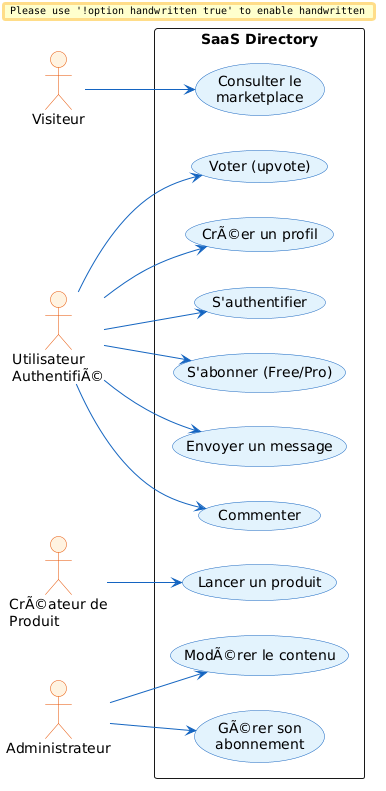
\includegraphics[width=0.95\textwidth]{assets/use_case.png}

\caption{Diagramme de Cas d'Utilisation — SaaS Directory}

\label{fig:use-case}

\end{figure}



La figure~\ref{fig:use-case} illustre les relations entre les quatre acteurs principaux et les cas d'utilisation du système. Le visiteur non authentifié peut consulter le marketplace. Une fois authentifié, l'utilisateur accède à l'ensemble des fonctionnalités sociales (votes, commentaires, messages). Le créateur de produit bénéficie de capacités de publication. L'administrateur dispose de privilèges de modération.



\subsubsection{Diagramme de Classes}



Le schéma Drizzle ORM dans \texttt{src/lib/db/schema.ts} constitue l'implémentation directe du diagramme de classes. Le système compte 20 tables regroupées en trois catégories.



\begin{figure}[H]

\centering

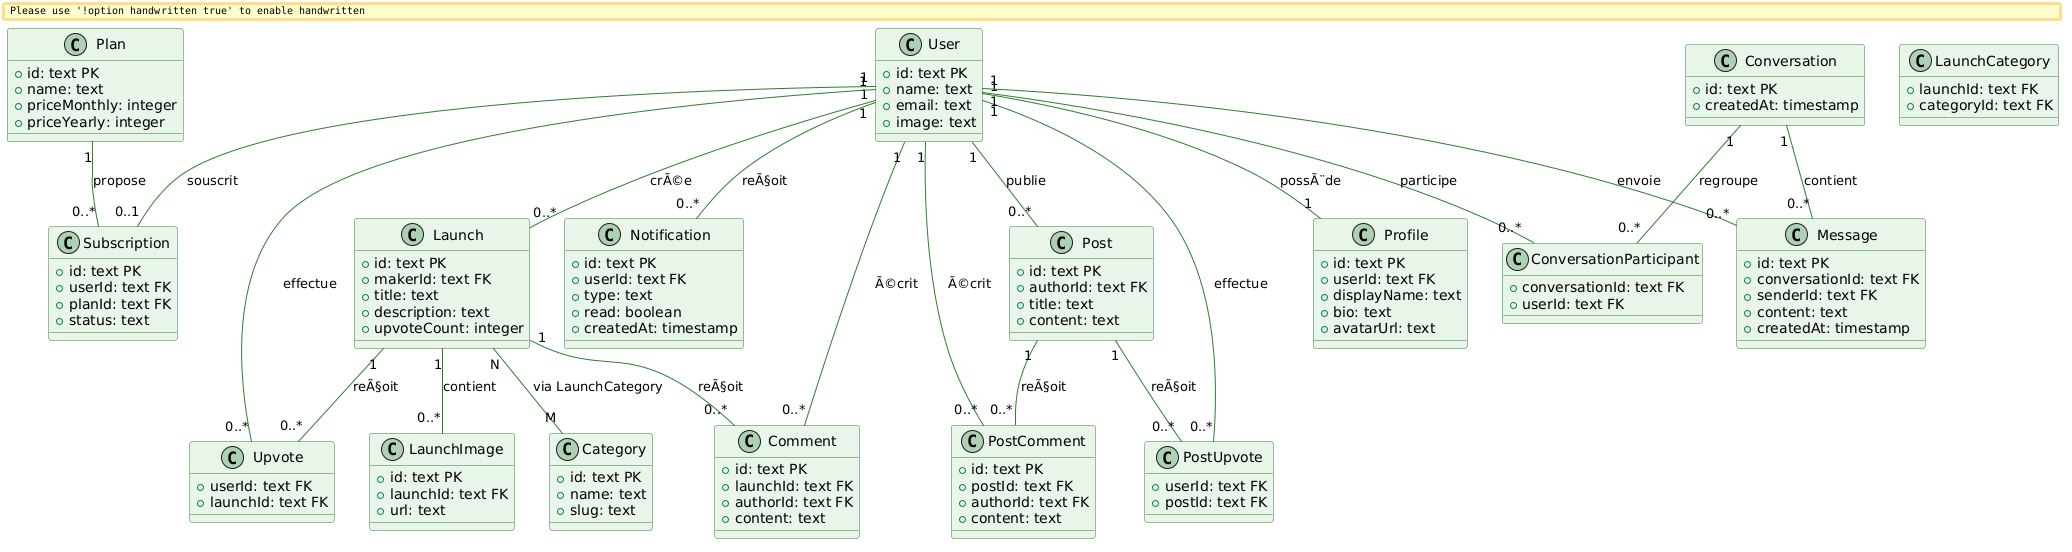
\includegraphics[width=0.95\textwidth]{assets/class.png}

\caption{Diagramme de Classes — SaaS Directory (20 tables)}

\label{fig:class}

\end{figure}



La figure~\ref{fig:class} présente l'architecture des classes avec leurs attributs et relations. Les \textbf{tables Better Auth} (\texttt{user}, \texttt{session}, \texttt{account}, \texttt{verification}) gèrent l'authentification. Les \textbf{tables métier principales} (\texttt{profile}, \texttt{launch}, \texttt{category}, \texttt{plan}, \texttt{subscription}) modélisent le cÅ“ur du marketplace. Les \textbf{tables d'interaction sociale} (\texttt{upvote}, \texttt{comment}, \texttt{post}, \texttt{postUpvote}, \texttt{postComment}, \texttt{conversation}, \texttt{conversationParticipant}, \texttt{message}, \texttt{notification}) gèrent la dynamique communautaire.



Les relations entre ces entités suivent le modèle relationnel classique : \texttt{User} possède un \texttt{Profile} (1:1), \texttt{User} crée des \texttt{Launches} (1:N), \texttt{Launch} appartient à des \texttt{Categories} (N:M via \texttt{launchCategory}), \texttt{User} reçoit des \texttt{Notifications} (1:N), et \texttt{User} participe à des \texttt{Conversations} (N:M via \texttt{conversationParticipant}).



\subsubsection{Diagramme de Séquence}



Le diagramme de séquence de la messagerie temps réel illustre l'interaction entre les acteurs et le système.



\begin{figure}[H]

\centering

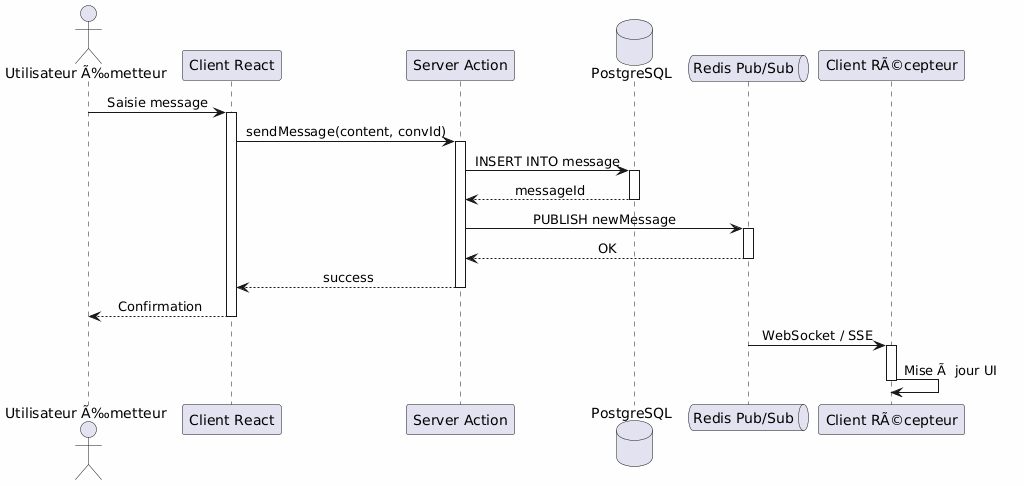
\includegraphics[width=0.95\textwidth]{assets/sequence.png}

\caption{Diagramme de Séquence — Envoi d'un Message en Temps Réel}

\label{fig:sequence}

\end{figure}



La figure~\ref{fig:sequence} montre le flux complet d'un message : l'utilisateur émetteur saisit le message via l'interface React. Le Client Component appelle la Server Action \texttt{sendMessage} qui insère le message dans la table \texttt{message} via Drizzle ORM. La Server Action publie ensuite un événement sur Redis Pub/Sub. Le serveur Redis notifie tous les clients abonnés à la conversation. Le Client Component récepteur reçoit la notification via WebSocket/SSE et met à jour l'interface sans rechargement de page. Ce flux démontre la séparation des préoccupations entre présentation, métier et persistance.



\subsection{Méthodes Formelles et Langage Z}



Les méthodes formelles (langage Z, B, VDM) utilisent des notations mathématiques pour spécifier, développer et vérifier des systèmes logiciels. Elles garantissent la correction du logiciel, éliminent les erreurs et facilitent la maintenance. Le langage Z, développé à l'Université d'Oxford par Jean-Raymond Abrial, est un langage de spécification formelle basé sur la théorie des ensembles, la logique des prédicats et un langage schématique pour structurer les spécifications.



Bien que puissantes, les méthodes formelles n'ont pas été utilisées dans ce projet pour plusieurs raisons pragmatiques. Premièrement, le domaine du marketplace web n'est pas critique au sens des systèmes embarqués ou médicaux où les méthodes formelles sont indispensables. Deuxièmement, la courbe d'apprentissage du langage Z est élevée et incompatible avec les contraintes temporelles d'un projet académique. Troisièmement, TypeScript et Zod fournissent un niveau de vérification formelle suffisant pour notre contexte (typage statique, validation de schémas à la compilation et à l'exécution).



Néanmoins, la compréhension des méthodes formelles reste essentielle pour apprécier les limites des approches semi-formelles et identifier les contextes où elles deviennent nécessaires.



% Chapitre 5 : La Normalisation

\section{Chapitre 5 : La Normalisation}



Les normes sont des apports documentés contenant des spécifications techniques ou autres critères précis destinés à être utilisés systématiquement en tant que règles, lignes directrices ou définitions des caractéristiques pour assurer que des matériaux, produits, processus et services sont aptes à leurs emplois.



\subsection{La Norme ISO et la Certification ISO 9000}



L'International Organization for Standardization (ISO), créée en 1947, est une fédération mondiale d'organismes nationaux de normalisation. La norme ISO 9000 traduit la démarche qualité au niveau de l'entreprise et apporte : en interne, l'amélioration de la compétitivité et la diminution des coûts ; à l'extérieur, la réponse aux exigences des donneurs d'ordre.



Pour mettre en Å“uvre une norme ISO 9000, il faut réaliser un diagnostic de l'organisation en auditant les fonctions principales. Les points nécessaires incluent : la gestion documentaire, la revue du contrat, la gestion des produits non-conformes, et la traçabilité. Dans le contexte de SaaS Directory, la gestion documentaire est assurée par les fichiers README.md, AGENTS.md, et les conventions de commit Git. La traçabilité est garantie par l'historique Git et les migrations Drizzle numérotées (0000 à 0003).



\subsection{Les Normes IEEE}



L'Institute of Electrical and Electronics Engineers (IEEE) a défini un ensemble de 37 normes s'intéressant aux processus, produits et techniques de base du génie logiciel. Trois normes sont particulièrement pertinentes pour notre projet.



\begin{definitionbox}[title={IEEE Std 12207.0}]

Fixe la signification des termes et choisit les processus prioritaires du cycle de vie du logiciel. Peut être considérée comme un dictionnaire et une liste de vérification pour la gestion des projets.

\end{definitionbox}



\begin{definitionbox}[title={IEEE Std 830}]

Recommandée pour les spécifications des exigences du logiciel. Pourrait être intégrée avec les approches de validation par prototype.

\end{definitionbox}



\begin{definitionbox}[title={IEEE Std 1028}]

Pour appliquer la validation et la vérification. Norme facilement adaptable à tous les problèmes.

\end{definitionbox}



L'application de ces normes à SaaS Directory se concrétise par : la définition claire des exigences fonctionnelles (authentification, marketplace, messagerie, monétisation) conformément à l'IEEE 830 ; la revue systématique du code via les pull requests Git, alignée avec l'IEEE 1028 ; et la traçabilité des exigences à travers les tests end-to-end Playwright, en accord avec l'IEEE 12207.0.



\subsection{Normalisation Appliquée au Projet}



\subsubsection{Normes de Codage}



Le projet respecte des conventions strictes de normalisation du code source. Les normes de nommage sont systématiquement appliquées : PascalCase pour les composants React (\texttt{UserCard.tsx}, \texttt{ProductForm.tsx}), camelCase pour les fonctions et variables (\texttt{sendMessage()}, \texttt{upvoteCount}), et kebab-case pour les routes API (\texttt{/api/messages/send}). Les imports sont organisés par groupe : React/Next.js, bibliothèques tierces, composants internes, utilitaires. Cette normalisation facilite la revue de code et réduit les conflits de fusion.



\subsubsection{Architecture Normalisée}



L'architecture suit le pattern MVC (Model-View-Controller) adapté à Next.js 16.2.4. Le \textbf{Modèle} est constitué par le schéma Drizzle ORM (\texttt{src/lib/db/schema.ts}) et les fonctions d'accès aux données. La \textbf{Vue} est implémentée par les composants React et les Server Components de Next.js. Le \textbf{Contrôleur} est assuré par les Server Actions (\texttt{src/lib/actions/}) qui encapsulent la logique métier. Cette séparation claire respecte les principes SOLID et facilite les tests unitaires.



\subsubsection{Gestion Documentaire et Traçabilité}



La gestion documentaire est assurée par plusieurs artefacts. Le fichier README.md présente le projet, son installation et son utilisation. Le fichier AGENTS.md documente les conventions spécifiques pour les agents de développement. Le fichier package.json liste l'ensemble des dépendances avec leurs versions exactes (Next.js 16.2.4, React 19.2.4, Drizzle ORM 0.45.2, etc.). Les commits Git suivent une convention descriptive (\texttt{feat:}, \texttt{fix:}, \texttt{chore:}). Les migrations Drizzle sont numérotées séquentiellement (0000 à 0003) et documentées, garantissant la traçabilité complète de l'évolution du schéma de base de données.



% Chapitre 6 : Les Tests

\section{Chapitre 6 : Les Tests}



Les tests logiciels constituent une phase critique du cycle de vie du logiciel, visant à détecter les erreurs et à garantir que le système répond aux exigences fonctionnelles et non-fonctionnelles spécifiées.



\subsection{Types de Tests et Stratégie}



La stratégie de tests de SaaS Directory repose sur une pyramide de tests classique, adaptée à l'architecture moderne de Next.js 16.2.4.



\subsubsection{Tests Unitaires}



Les tests unitaires sont implémentés avec Vitest 4.1.5, un framework de test rapide compatible avec Vite et Next.js. Onze fichiers de test couvrent l'authentification (\texttt{auth-client.test.ts}), la souscription (\texttt{subscription.test.ts}), le schéma Drizzle (\texttt{schema.test.ts}), les actions serveur (\texttt{post.test.ts}, \texttt{launch.test.ts}, \texttt{message.test.ts}), et les composants UI (\texttt{theme-toggle.test.tsx}, \texttt{infrastructure.test.tsx}, \texttt{page.test.tsx} pour login et signup).



Ces tests vérifient le comportement isolé des fonctions et composants, sans dépendances externes. Par exemple, \texttt{schema.test.ts} valide que toutes les colonnes attendues existent dans chaque table, et que les contraintes de clé étrangère sont correctement définies.



\subsubsection{Tests d'Intégration et End-to-End}



Les tests end-to-end sont réalisés avec Playwright 1.59.1, un outil moderne de test d'interface automatisé. La configuration (\texttt{playwright.config.ts}) définit un projet Chromium avec tracing activé. Le fichier \texttt{e2e/homepage.spec.ts} teste le parcours utilisateur critique : navigation, authentification, et affichage du marketplace.



Ces tests vérifient l'intégration complète du système : le frontend React, les Server Actions, l'ORM Drizzle, et la base PostgreSQL. Ils s'exécutent contre une instance locale du serveur de développement Next.js.



\subsubsection{Tests de Performance}



La performance est évaluée par l'optimisation des requêtes Drizzle ORM et la configuration des indexes PostgreSQL. Le projet inclut un script de benchmark pour le cache Redis (\texttt{scripts/benchmark-cache.ts}) qui mesure les temps de réponse du cache par rapport aux requêtes directes en base de données.



\subsection{Outils et Environnement de Test}



L'environnement de test de SaaS Directory est entièrement dockerisé. Le fichier \texttt{docker-compose.test.yml} définit un environnement isolé comprenant une base PostgreSQL de test sur le port 5433, et l'application Next.js en mode test.



La séparation des environnements (développement, test, production) est assurée par les variables d'environnement : \texttt{DATABASE\_URL} pour le développement, \texttt{DATABASE\_URL\_TEST} pour les tests. Cette isolation garantit que les tests ne perturbent jamais les données de développement.



\subsection{Couverture et Résultats}



La couverture de tests cible les fonctions critiques du système : l'authentification (création de compte, connexion, 2FA, gestion de session), la gestion des rôles (administrateur vs utilisateur standard), le marketplace (création de produit, vote, commentaire), la messagerie (envoi, réception, marquage comme lu), et les abonnements (souscription, changement de plan, annulation).



Les seuils de couverture sont configurés dans \texttt{vitest.config.ts} avec un minimum de 70\% pour les branches et les fonctions. Ce seuil est réaliste pour un projet académique tout en garantissant un niveau de qualité professionnel.



% Chapitre 7 : La Gestion des Projets Logiciels

\section{Chapitre 7 : La Gestion des Projets Logiciels}



La gestion des projets logiciels vise à structurer méthodiquement et progressivement une réalité à venir, en appliquant un objectif et des actions à entreprendre avec des ressources données. Le rôle du chef de projet est de planifier, organiser et contrôler l'ensemble des activités nécessaires à la réalisation du projet.



\subsection{Organisation du Projet (WBS, PBS, OBS)}



Trois outils structurants ont guidé l'organisation du projet.



Le \textbf{Work Breakdown Structure (WBS)} décompose le projet en tâches hiérarchiques. Pour SaaS Directory, le WBS s'articule autour de cinq phases principales (fondations, profil, marketplace, messagerie, monétisation), chacune subdivisée en tâches techniques (développement frontend, développement backend, tests, documentation).



Le \textbf{Product Breakdown Structure (PBS)} identifie les livrables de chaque phase : authentification fonctionnelle, profil utilisateur opérationnel, produit lancable sur le marketplace, système de messagerie temps réel, et système d'abonnements Free/Pro.



Le \textbf{Organizational Breakdown Structure (OBS)} répartit les responsabilités. Le projet a été réalisé par deux développeurs en binôme, avec une répartition naturelle des tâches selon les compétences (frontend React vs backend Server Actions).



\subsection{Planification (GANTT, PERT)}



La planification du projet a utilisé un diagramme de GANTT pour visualiser les cinq phases sur une échelle temporelle. Chaque phase correspond à un sprint de développement d'environ trois à quatre semaines, avec des jalons intermédiaires (MVP marketplace, messagerie fonctionnelle).



\begin{figure}[H]

\centering

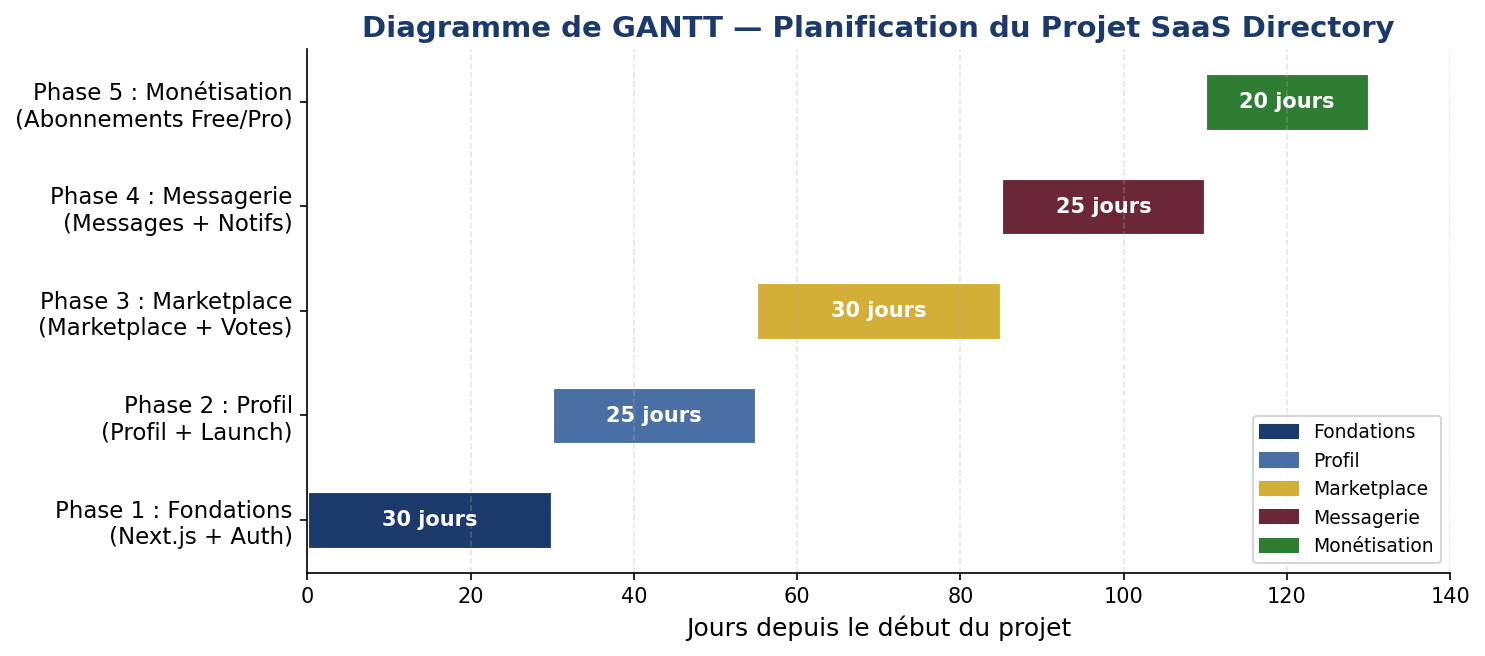
\includegraphics[width=0.95\textwidth]{assets/gantt.png}

\caption{Diagramme de GANTT — Planification du Projet SaaS Directory}

\label{fig:gantt}

\end{figure}



La figure~\ref{fig:gantt} présente la répartition temporelle des cinq phases du projet sur une échelle de 130 jours. La Phase 1 (Fondations) occupe les 30 premiers jours, suivie par le Profil (25 jours), le Marketplace (30 jours), la Messagerie (25 jours), et enfin la Monétisation (20 jours).



Le diagramme PERT (Program Evaluation and Review Technique) modélise les dépendances entre tâches. Les liaisons principales sont de type "fin à début" : l'authentification (Phase 1) doit être terminée avant le profil (Phase 2) ; le profil avant le marketplace (Phase 3) ; le marketplace avant la messagerie (Phase 4) ; la messagerie avant la monétisation (Phase 5).



\subsection{Estimation des Coûts par COCOMO}



L'estimation des coûts d'un projet logiciel est un exercice délicat. Les raisons classiques de dépassement incluent l'optimisme, la négligence des problèmes techniques, le manque d'expérience, l'oubli de la documentation, et la sous-estimation des tâches annexes. Pour contrer ces biais, nous avons appliqué la méthode COCOMO (COnstructive COst MOdel) de Barry Boehm, un modèle d'estimation empirique basé sur la taille du projet en KLOC.



\subsubsection{Taille du Projet}



Le codebase de SaaS Directory compte 12 166 lignes de code réparties sur 108 fichiers TypeScript/TSX, soit approximativement 14 KLOC. Cette taille inclut le code source applicatif (\texttt{src/app} : 3 198 LOC, \texttt{src/components} : 5 234 LOC, \texttt{src/lib} : 2 957 LOC), les tests (\texttt{src/test} : 111 LOC, \texttt{e2e} : 33 LOC), et les scripts (1 115 LOC).



\subsubsection{Application du COCOMO de Base}



Pour un projet web moderne avec une stack technologique récente (Next.js 16.2.4, React 19.2.4, TypeScript 5), nous avons retenu le mode semi-détaché (projet moyennement complexe, équipe avec expérience mixte, contraintes modérées). Les coefficients du mode semi-détaché sont $a = 3{,}0$ et $b = 1{,}12$.



\begin{table}[H]

\centering

\caption{Estimation COCOMO de Base — Mode Semi-Détaché (14 KLOC)}

\label{tab:cocomo}

\begin{tabular}{@{}lll@{}}

\toprule

\textbf{Paramètre} & \textbf{Formule / Valeur} & \textbf{Résultat} \\

\midrule

Taille du projet & 12 166 LOC $\approx$ 14 KLOC & 14 KLOC \\

Mode de développement & Semi-Détaché & $a = 3{,}0$ ; $b = 1{,}12$ \\

Effort estimé & $E = a \times (\text{KLOC})^b$ & $E \approx 58$ Personnes-Mois \\

Durée estimée & $D = 2{,}5 \times E^{0{,}35}$ & $D \approx 9{,}5$ mois \\

Taille d'équipe théorique & $N = E / D$ & $N \approx 6$ personnes \\

\midrule

\textbf{Taille d'équipe réelle} & \textbf{2 développeurs sur 5 mois} & \textbf{10 Personnes-Mois} \\

\bottomrule

\end{tabular}

\end{table}



Ces chiffres constituent une estimation théorique à visée pédagogique. En réalité, le projet a été réalisé par deux développeurs travaillant en parallèle sur une période académique d'environ cinq mois, soit environ 10 Personnes-Mois. Cet écart illustre la différence fréquente entre les modèles prédictifs et la réalité des projets académiques en mode agile.



% Chapitre 8 : L'Analyse des Risques

\section{Chapitre 8 : L'Analyse des Risques}



L'analyse des risques est une composante essentielle de la conduite de projet. Elle vise à identifier, évaluer et traiter les événements incertains qui pourraient affecter négativement les objectifs du projet.



\subsection{Identification des Risques}



L'identification des risques a été réalisée par une analyse systématique des dimensions techniques, sécuritaires et opérationnelles du projet. Trois catégories principales de risques ont été identifiées.



\subsubsection{Risques Techniques}



Le risque technique majeur réside dans la complexité de Next.js 16.2.4 avec le App Router. Ce framework, bien que puissant, introduit des breaking changes significatifs par rapport aux versions précédentes. La documentation évolue rapidement, et certaines fonctionnalités (Server Actions, Parallel Routes, Intercepting Routes) sont encore relativement nouvelles et peu documentées.



Un risque secondaire concerne la stack Drizzle ORM 0.45.2 + PostgreSQL. Bien que mature, la configuration des relations et des indexes nécessite une expertise SQL approfondie pour garantir les performances à grande échelle.



\subsubsection{Risques de Sécurité}



Les risques de sécurité concernent la protection des données utilisateurs et la prévention des attaques. L'injection SQL est mitigée par l'utilisation de Drizzle ORM avec des requêtes paramétrées, mais les Server Actions exposent des surfaces d'attaque potentielles si les validations côté serveur sont insuffisantes.



Les risques liés à l'authentification incluent la fuite de tokens JWT, la compromission des sessions, et les attaques par force brute. Better Auth 1.6.9 gère nativement plusieurs de ces menaces (expiration des tokens, rotation, rate limiting), mais la configuration incorrecte reste un risque.



\subsubsection{Risques de Performance}



Les risques de performance se manifestent à plusieurs niveaux. Le marketplace doit supporter un grand nombre de produits sans dégradation du temps de réponse, ce qui nécessite l'optimisation des indexes PostgreSQL et potentiellement l'ajout de pagination côté serveur. La messagerie temps réel via Redis Pub/Sub doit supporter un volume croissant de messages simultanés sans latence perceptible.



\subsection{Analyse et Stratégies de Mitigation}



Pour chaque risque identifié, une stratégie de mitigation a été définie et mise en Å“uvre.



\subsubsection{Mitigation des Risques Techniques}



La mitigation des risques techniques repose sur trois piliers. Premièrement, la veille technologique : le fichier AGENTS.md et la documentation officielle de Next.js sont consultés régulièrement pour anticiper les breaking changes. Deuxièmement, les tests end-to-end Playwright 1.59.1 détectent les régressions fonctionnelles avant qu'elles n'atteignent la branche master. Troisièmement, la modularité de l'architecture facilite le remplacement d'une technologie si elle devient obsolète.



\subsubsection{Mitigation des Risques de Sécurité}



La sécurité est assurée par plusieurs mécanismes de défense en profondeur. L'authentification Better Auth gère nativement la sécurité des sessions (tokens JWT, expiration, rotation). Les Server Actions valident systématiquement les entrées utilisateur via Zod 4.4.3. Les indexes PostgreSQL accélèrent les requêtes fréquentes (recherche par email, par slug, par catégorie) tout en limitant la surface d'attaque par injection.



\subsubsection{Mitigation des Risques de Performance}



La performance est optimisée par plusieurs techniques. Les indexes PostgreSQL sont définis dans le schéma Drizzle pour accélérer les requêtes fréquentes (recherche par email, par slug, par catégorie). Le cache Redis réduit la charge sur la base de données pour les données fréquemment accédées (sessions, profils, listes de catégories). La pagination côté serveur est implémentée pour le marketplace et la messagerie, évitant le chargement de volumes excessifs de données.



\subsection{Plan de Continuité}



En cas d'incident majeur, le plan de continuité prévoit plusieurs mesures. La restauration depuis les backups PostgreSQL est la première ligne de défense. Le système de migrations Drizzle permet de reconstruire le schéma de base de données à partir de zéro. Le versioning Git (branche master + tags) permet de revenir à une version stable du code en cas de déploiement problématique. La documentation technique (README.md, AGENTS.md) facilite l'onboarding d'un nouveau développeur en cas d'indisponibilité d'un membre de l'équipe.



% Chapitre 9 : Conduite du Changement

\section{Chapitre 9 : Conduite du Changement}



La conduite du changement est la discipline qui vise à accompagner les transformations au sein d'un projet ou d'une organisation, en minimisant les résistances et en maximisant l'adhésion des parties prenantes.



\subsection{Nature des Changements}



Plusieurs types de changements ont affecté le projet tout au long de son développement. Les \textbf{changements technologiques} incluent la mise à jour de Next.js 15 vers Next.js 16.2.4 (breaking changes sur le App Router), la migration de Tailwind CSS v3 vers v4 (nouvelle syntaxe de configuration), et l'ajout de Redis pour la messagerie temps réel (architecture initialement prévue sans cache dédié).



Les \textbf{changements fonctionnels} concernent l'ajout de fonctionnalités non prévues initialement : le système de notifications temps réel, l'édition et la suppression des commentaires, et le système de pagination infinie pour la messagerie.



Les \textbf{changements organisationnels} touchent la répartition des tâches entre les deux développeurs, avec des ajustements selon les compétences et les disponibilités de chacun.



\subsection{Gestion des Versions}



Le contrôle de versions est assuré par Git avec une stratégie de branches structurée. La branche \texttt{master} constitue la version de production, stable et déployée. Les branches de fonctionnalités (\texttt{feature/auth-2fa}, \texttt{feature/messaging}, etc.) isolent le développement des nouvelles fonctionnalités. Les pull requests obligatoires avec revue de code assurent la qualité avant fusion.



Les migrations Drizzle constituent un mécanisme de gestion du changement au niveau de la persistance. Chaque migration est un fichier SQL versionné (\texttt{0000\_remarkable\_carnage.sql}, \texttt{0001\_cuddly\_namora.sql}, \texttt{0002\_add\_logo\_url\_to\_launch.sql}, \texttt{0003\_groovy\_hannibal\_king.sql}) qui peut être appliquée et, si nécessaire, revertée. Cette approche garantit la cohérence du schéma de base de données entre les environnements de développement, test et production.



\subsection{Adaptation et Communication}



L'architecture modulaire du projet a facilité l'adaptation aux changements. L'ajout du champ \texttt{logoUrl} dans la table \texttt{Launch} (migration 0002) n'a nécessité que la modification d'un seul fichier de schéma et de quelques lignes dans le composant frontend. Le passage à Next.js 16.2.4 a été géré par la lecture attentive de la documentation de migration officielle et des tests end-to-end Playwright qui ont validé l'absence de régressions.



La communication autour des changements repose sur plusieurs canaux. La documentation technique (README.md, AGENTS.md) est maintenue à jour après chaque changement majeur. Les messages de commit Git suivent une convention descriptive (\texttt{feat:}, \texttt{fix:}, \texttt{chore:}) qui facilite la génération de changelog. Les discussions techniques sont documentées dans les pull requests, créant une base de connaissances consultable pour les décisions architecturales passées.





% ======================== CONCLUSION ========================

\section*{Conclusion Générale et Perspectives}

\addcontentsline{toc}{section}{Conclusion Générale et Perspectives}



Ce rapport a présenté l'application systématique des concepts de Génie Logiciel et de Conduite de Projet au développement de SaaS Directory. Du point de vue du cycle de vie, le modèle incrémental itératif adopté a permis de livrer cinq versions fonctionnelles successives, chacune apportant une valeur métier concrète.



La démarche orientée objet, matérialisée par le schéma Drizzle ORM de 20 tables et les composants React modulaires, assure la maintenabilité et l'évolutivité du système. Les cinq diagrammes UML (cas d'utilisation, classes, séquence, déploiement, GANTT) fournissent une documentation visuelle complète du projet.



La gestion de projet, illustrée par le WBS en cinq phases, le diagramme de GANTT, et l'estimation COCOMO, démontre la faisabilité d'une planification rigoureuse même dans un contexte académique. L'analyse des risques a permis d'anticiper et de mitiger les principales menaces techniques et sécuritaires.



L'utilisation d'une stack technologique moderne et cohérente — Next.js 16.2.4, React 19.2.4, TypeScript 5, Tailwind CSS v4, Drizzle ORM 0.45.2, Better Auth 1.6.9, PostgreSQL, et Redis — a grandement facilité le développement et garanti la qualité du livrable final.



Les perspectives d'évolution de SaaS Directory sont nombreuses. L'intégration complète de Stripe pour le paiement (le schéma contient déjà les champs stripeCustomerId et stripeSubscriptionId), l'ajout d'un système de recherche avancée avec Elasticsearch, et le déploiement sur une infrastructure cloud avec Docker et Kubernetes constituent les axes de développement futurs.



\newpage



% ======================== BIBLIOGRAPHY ========================

\section*{Bibliographie et Webographie}

\addcontentsline{toc}{section}{Bibliographie et Webographie}



\begin{itemize}[leftmargin=1.5em]

\item Barry Boehm, \textit{Software Engineering Economics}, Prentice-Hall, 1977.

\item Grady Booch, \textit{Object-Oriented Analysis and Design with Applications}, 2nd Edition, Benjamin/Cummings, 1994.

\item Jean-Raymond Abrial, \textit{The B-Book: Assigning Programs to Meanings}, Cambridge University Press, 1996.

\item ISO/IEC 12207:2017, Systems and software engineering — Software life cycle processes.

\item IEEE Std 830-1998, IEEE Recommended Practice for Software Requirements Specifications.

\item IEEE Std 1028-2008, IEEE Standard for Software Reviews and Audits.

\item IEEE Std 12207.0-1996, IEEE Standard for Information Technology — Software life cycle processes.

\item Cours de Génie Logiciel et Conduite de Projet, Année Universitaire 2025-2026.

\item Next.js Documentation, \url{https://nextjs.org/docs}, consulté en 2026.

\item React Documentation, \url{https://react.dev}, consulté en 2026.

\item Drizzle ORM Documentation, \url{https://orm.drizzle.team}, consulté en 2026.

\item Better Auth Documentation, \url{https://www.better-auth.com}, consulté en 2026.

\item Tailwind CSS Documentation, \url{https://tailwindcss.com}, consulté en 2026.

\item PostgreSQL Documentation, \url{https://www.postgresql.org/docs}, consulté en 2026.

\item Redis Documentation, \url{https://redis.io/documentation}, consulté en 2026.

\item Vitest Documentation, \url{https://vitest.dev}, consulté en 2026.

\item Playwright Documentation, \url{https://playwright.dev}, consulté en 2026.

\end{itemize}



\newpage



% ======================== ANNEXES ========================

% Annexes

\section*{Annexes}

\addcontentsline{toc}{section}{Annexes}



\subsection*{Annexe A : Schéma de la Base de Données Drizzle ORM}

\addcontentsline{toc}{subsection}{Annexe A : Schéma de la Base de Données}



Cette annexe présente un extrait du schéma Drizzle ORM (\texttt{src/lib/db/schema.ts}) illustrant la structure des tables principales.



\begin{codebox}

\begin{lstlisting}

// Tables Better Auth (authentification)

export const user = pgTable("user", {

  id: text("id").primaryKey(),

  name: text("name"),

  email: text("email").notNull().unique(),

  emailVerified: boolean("email_verified").default(false),

  image: text("image"),

  createdAt: timestamp("created_at").defaultNow(),

  updatedAt: timestamp("updated_at").defaultNow(),

});



export const session = pgTable("session", {

  id: text("id").primaryKey(),

  userId: text("user_id").notNull().references(() => user.id),

  token: text("token").notNull().unique(),

  expiresAt: timestamp("expires_at").notNull(),

});



export const account = pgTable("account", {

  id: text("id").primaryKey(),

  userId: text("user_id").notNull().references(() => user.id),

  accountId: text("account_id").notNull(),

  providerId: text("provider_id").notNull(),

});



export const verification = pgTable("verification", {

  id: text("id").primaryKey(),

  identifier: text("identifier").notNull(),

  value: text("value").notNull(),

  expiresAt: timestamp("expires_at").notNull(),

});



// Table profile (1:1 avec user)

export const profile = pgTable("profile", {

  id: serial("id").primaryKey(),

  userId: text("user_id").notNull().references(() => user.id).unique(),

  displayName: text("display_name"),

  bio: text("bio"),

  website: text("website"),

  twitter: text("twitter"),

  github: text("github"),

  avatarUrl: text("avatar_url"),

});



// Table launch (produit SaaS)

export const launch = pgTable("launch", {

  id: serial("id").primaryKey(),

  makerId: text("maker_id").notNull().references(() => user.id),

  title: text("title").notNull(),

  description: text("description"),

  logoUrl: text("logo_url"),

  upvoteCount: integer("upvote_count").default(0),

  createdAt: timestamp("created_at").defaultNow(),

});



// Table category

export const category = pgTable("category", {

  id: serial("id").primaryKey(),

  name: text("name").notNull(),

  slug: text("slug").notNull().unique(),

});



// Table plan (Free / Pro)

export const plan = pgTable("plan", {

  id: serial("id").primaryKey(),

  name: text("name").notNull(),

  priceMonthly: integer("price_monthly"),

  priceYearly: integer("price_yearly"),

  stripeProductId: text("stripe_product_id"),

  stripeMonthlyPriceId: text("stripe_monthly_price_id"),

  stripeYearlyPriceId: text("stripe_yearly_price_id"),

});



// Table subscription

export const subscription = pgTable("subscription", {

  id: serial("id").primaryKey(),

  userId: text("user_id").notNull().references(() => user.id).unique(),

  planId: integer("plan_id").notNull().references(() => plan.id),

  status: text("status").notNull().default("active"),

  stripeCustomerId: text("stripe_customer_id"),

  stripeSubscriptionId: text("stripe_subscription_id"),

});

\end{lstlisting}

\end{codebox}



\newpage



\subsection*{Annexe B : Structure du Projet}

\addcontentsline{toc}{subsection}{Annexe B : Structure du Projet}



\begin{codebox}

\begin{lstlisting}

marketplace-saas/ (12 166 LOC, 108 fichiers)

|-- e2e/                        (33 LOC)

|   |-- homepage.spec.ts

|-- public/

|   |-- uploads/launches/

|-- src/

|   |-- app/                    (3 198 LOC)

|   |   |-- layout.tsx

|   |   |-- page.tsx

|   |   |-- about/, api/, contact/, feed/

|   |   |-- forgot-password/, launch/, login/

|   |   |-- marketplace/, messages/, my-launches/

|   |   |-- new/, notifications/, pricing/

|   |   |-- privacy/, profile/, reset-password/

|   |   |-- settings/, signup/, terms/

|   |-- components/             (5 234 LOC)

|   |   |-- auth/, dev/, feed/, launch/

|   |   |-- marketplace/, providers/, ui/

|   |-- hooks/

|   |-- lib/                    (2 957 LOC)

|   |   |-- actions/            (Server Actions)

|   |   |-- db/

|   |   |   |-- migrations/     (4 migrations)

|   |   |   |   |-- 0000_remarkable_carnage.sql

|   |   |   |   |-- 0001_cuddly_namora.sql

|   |   |   |   |-- 0002_add_logo_url_to_launch.sql

|   |   |   |   |-- 0003_groovy_hannibal_king.sql

|   |   |   |-- schema.ts       (20 tables)

|   |   |   |-- index.ts

|   |   |-- auth.ts, auth-client.ts

|   |   |-- cache.ts, subscription.ts

|   |   |-- upload.ts, utils.ts

|   |   |-- *.test.ts           (11 fichiers de test)

|   |-- test/                   (111 LOC)

|   |-- types/

|-- next.config.ts

|-- package.json

|-- tsconfig.json

|-- vitest.config.ts

|-- playwright.config.ts

|-- drizzle.config.ts

|-- docker-compose.test.yml

\end{lstlisting}

\end{codebox}



\newpage



\subsection*{Annexe C : Dépendances Principales}

\addcontentsline{toc}{subsection}{Annexe C : Dépendances Principales}



\begin{table}[H]

\centering

\caption{Dépendances principales du projet SaaS Directory}

\label{tab:deps}

\begin{tabular}{@{}lll@{}}

\toprule

\textbf{Dépendance} & \textbf{Version} & \textbf{Description} \\

\midrule

next & 16.2.4 & Framework React avec App Router \\

react & 19.2.4 & Bibliothèque UI \\

react-dom & 19.2.4 & Rendu DOM React \\

drizzle-orm & 0.45.2 & ORM type-safe pour PostgreSQL \\

better-auth & 1.6.9 & Authentification OAuth + 2FA \\

pg & 8.20.0 & Driver PostgreSQL \\

@tanstack/react-query & 5.100.9 & Gestion de cache et requêtes \\

zod & 4.4.3 & Validation de schémas \\

framer-motion & 12.38.0 & Animations React \\

ioredis & 5.10.1 & Client Redis \\

resend & 6.12.2 & Service d'envoi d'emails \\

sonner & 2.0.7 & Notifications toast UI \\

tailwindcss & 4.0.0 & Framework CSS utilitaire \\

typescript & 5.7.0 & Typage statique \\

vitest & 4.1.5 & Tests unitaires et d'intégration \\

@playwright/test & 1.59.1 & Tests end-to-end \\

eslint & 9.0.0 & Linting du code \\

eslint-config-next & 16.2.4 & Règles ESLint Next.js \\

\bottomrule

\end{tabular}

\end{table}



\newpage



\subsection*{Annexe D : Diagramme de Déploiement}

\addcontentsline{toc}{subsection}{Annexe D : Diagramme de Déploiement}



\begin{figure}[H]

\centering

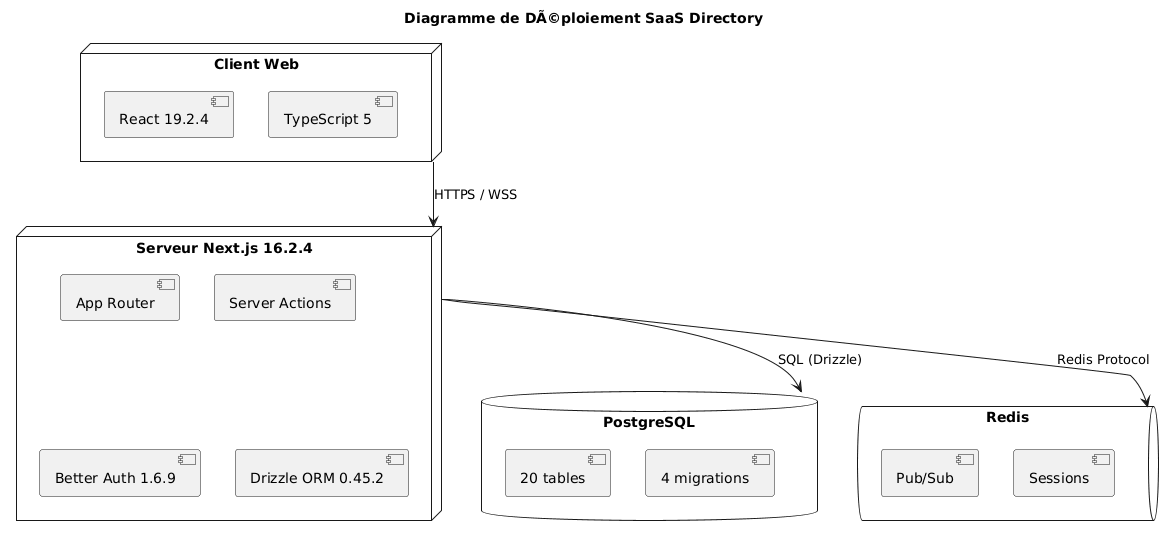
\includegraphics[width=0.95\textwidth]{assets/deployment.png}

\caption{Diagramme de Déploiement — Architecture Physique de SaaS Directory}

\label{fig:deployment}

\end{figure}



La figure~\ref{fig:deployment} décrit l'architecture physique du système et la répartition des artefacts logiciels sur les nÅ“uds matériels. SaaS Directory repose sur une architecture cloud-native distribuée sur trois environnements principaux : le client web (navigateur), la plateforme serverless (Next.js 16.2.4), et les services de données (PostgreSQL + Redis).



Le client web (React 19.2.4 / TypeScript 5) s'exécute dans le navigateur et communique avec les fonctions serverless via HTTPS. Les Server Actions Next.js 16.2.4 interagissent avec la base de données PostgreSQL via Drizzle ORM 0.45.2. Le système de messagerie temps réel utilise Redis Pub/Sub pour la diffusion des messages entre les instances serverless. L'authentification est assurée par Better Auth 1.6.9. Cette architecture sans serveur offre une scalabilité automatique et une réduction des coûts d'infrastructure.





\end{document}

